\documentclass[14pt,a4paper,final]{extreport}
\nonstopmode
\usepackage[T2A]{fontenc}
\usepackage[utf8]{inputenc}
\DeclareUnicodeCharacter{0306}{~}
\usepackage[russian]{babel}
\usepackage[a4paper, top=2cm, bottom=2cm, left=2cm, right=1cm,marginparsep=.5cm]{geometry}
\usepackage{fancyhdr}
\usepackage[export]{adjustbox}
\usepackage{marginnote}
\usepackage{tabularray}
\usepackage{longtable}
\usepackage{ltablex}
\usepackage{amsmath}    % Подключение пакета amsmath

\usepackage{caption}

% Настройка отображения заголовков рисунков
\captionsetup[figure]{name=Рисунок, labelsep=period, labelfont=bf}

\captionsetup[table]{name=Таблица, labelsep=period, labelfont=bf}

\usepackage{enumitem}
\setlist[itemize]{leftmargin=\parindent,nosep}
\setlist[enumerate]{leftmargin=\parindent,nosep}
\renewcommand\labelitemi{--}

\usepackage[none]{hyphenat}
\usepackage{setspace}
\onehalfspacing 
\usepackage{float}
\usepackage{xpatch}

\usepackage{tocloft, titlesec, titletoc}
\usepackage{indentfirst}
\titleformat{\chapter}[block]{\normalfont\bfseries\large}{\thechapter}{1ex}{\centering\MakeUppercase}
\titlespacing*{\chapter}{0pt}{-\baselineskip}{2\baselineskip}

\titleformat{\section}[block]{\normalfont}{\thesection}{1ex}{\normalfont}
\titlespacing{\section}{1.25cm}{\baselineskip}{\baselineskip}

%Оформление подразделов
\titleformat{\subsection}[block]{\normalfont}{\thesubsection}{1ex}{\normalfont}
\titlespacing{\subsection}{1.25cm}{\baselineskip}{\baselineskip}

%Оформление под-подразделов
\titleformat{\subsubsection}[block]{\normalfont}{\thesubsection}{1ex}{\normalfont}
\titlespacing{\subsubsection}{1.25cm}{0pt}{\baselineskip}

\usepackage{titlesec}

% Настройка глубины нумерации заголовков
\setcounter{secnumdepth}{3}
\setcounter{tocdepth}{3}

% Настройка внешнего вида заголовков с помощью titlesec
\titleformat{\subsubsection}[hang]{\normalfont\normalsize}{\thesubsubsection}{0.5em}{}

%\titlespacing{\subsubsection}{35pt}{\parskip}{\parskip}

%\setcounter{tocdepth}{4}%
%\setcounter{secnumdepth}{4}% Number \subsubsection
\renewcommand{\cftdotsep}{2.75}
\renewcommand{\cftchapfont}{\normalfont}
\renewcommand{\cfttoctitlefont}{\hfill\normalfont\large\bfseries}
\renewcommand{\cftaftertoctitle}{\hfill}
\renewcommand{\cftchapleader}{\cftdotfill{\cftdotsep}} % for chapters
\renewcommand{\cftsecleader}{\cftdotfill{\cftdotsep}}  % for sections
\renewcommand{\cftsubsecleader}{\cftdotfill{\cftdotsep}} % for subsections
\renewcommand{\cftsubsubsecleader}{\cftdotfill{\cftdotsep}} % for subsubsections
\setlength{\cftbeforetoctitleskip}{-.6\baselineskip}
\setlength{\cftaftertoctitleskip}{-\baselineskip}
\setlength{\cftbeforechapskip}{\baselineskip}
\renewcommand{\cftchappagefont}{}

\renewcommand{\contentsname}{СОДЕРЖАНИЕ\vspace{\baselineskip}}% (ГОСТ Р 7.0.11-2011, 4)
\addto{\captionsrussian}{\renewcommand{\bibname}{СПИСОК ИСПОЛЬЗОВАННОЙ ЛИТЕРАТУРЫ\bigskip}}

\makeatletter
\renewcommand\@biblabel[1]{#1.\ }
\makeatother

\let\mtcontentsname\contentsname\addto\captionsrussian{\typeout{foo}\renewcommand{\contentsname}{\MakeUppercase\mtcontentsname}}

\makeatletter
\patchcmd{\chapter}{\if@openright\cleardoublepage\else\clearpage\fi}{\vspace{3\baselineskip}}{}{}
\makeatother

\newcommand*\rot[1]{\rotatebox{90}{#1}}
\newlength{\rs}
\setlength{\rs}{.5mm}

\makeatletter
\AddEnumerateCounter{\asbuk}{\russian@alph}{щ}
\makeatother

\fancypagestyle{firststyle}
{
    \fancyhf{} % sets both header and footer to nothing
    \renewcommand{\headrulewidth}{0pt}
    \fancyfoot[C]{
    
        {\vspace{-\baselineskip}\normalfont\textbf{Москва 2026}}
    } 
}

\begin{document}
\pagenumbering{gobble}
\raggedbottom

%для изменения
\newcommand{\fullname}{Егоров Александр Владиславович}
\newcommand{\shname}{Егоров А.В.}
\newcommand{\grp}{М3О-225БВ-24}
\newcommand{\variant}{5} %номер варианта (если многозначный - уберите 0 в \cipher)
\newcommand{\fieldA}{\( \vec a = y^2 \vec i + z^2 \vec j + x^2 \vec k \)}
\newcommand{\fieldB}{\( \vec b = (2xy^3z + y) \vec i + (3x^2y^2z + x) \vec j + (x^2y^3 + 4z^3) \vec k \)}

\newcommand{\cipher}{643.02066606.000\variant}
\newcommand{\cipherlri}{643.02066606.\\000\variant}
\newcommand{\docstamp}{\cipher-01 81 01}
\newcommand{\doctitle}{Программа визуализации\\эквипотенциальных поверхностей\\и силовых линий}
\newcommand{\doctitleoneline}{Программа визуализации эквипотенциальных поверхностей и силовых линий}
\newcommand{\programtitle}{FieldViz}
\newcommand{\docname}{Пояснительная записка}
\thispagestyle{firststyle}
\begin{flushright}
	\noindent\textbf{\large УТВЕРЖДАЮ}\\
	Руководитель разработки\\
	\rule{2.5cm}{.6pt} к.т.н., доц. Машкин М. Н.\\
	<<\rule{7mm}{.6pt}>> \rule{3cm}{.6pt} 2026
\end{flushright}

\vfill\vfill

\begin{center}
\bfseries\large
\doctitle

\bigskip
Вариант \variant

\bigskip
\docname

\bigskip
Лист утверждения

\bigskip
\docstamp-ЛУ
\end{center}

\vfill

\begin{flushright}
	\noindent Исполнитель\\
	Студент группы \grp\\
	\rule{2.5cm}{.6pt} \shname\\
	<<\rule{7mm}{.6pt}>> \rule{3cm}{.6pt} 2026
\end{flushright}

\vfill

\reversemarginpar\marginpar{
    \begin{adjustbox}{angle=90}
        \small
        \begin{tblr}{
          colspec={|[\rs]m{25mm}|[\rs]m{35mm}|[\rs]m{25mm}|[\rs]m{25mm}|[\rs]m{35mm}|[\rs]},
          rowspec={|[\rs]Q[5mm]|[\rs]Q[7mm]|[\rs]},rowsep=0pt,colsep=0pt}
        Инв. № подл. & \centering Подпись и дата & Взам. инв. № & Инв. № дубл. & \centering Подпись и дата\\
           & & & &
        \end{tblr}
        \hspace{-1.85cm}
    \end{adjustbox}
}
\pagebreak

\thispagestyle{firststyle}

\begin{minipage}{.50\textwidth}
\textbf{\large УТВЕРЖДЕНО}
\docstamp-ЛУ
\end{minipage}

%\noindent\begin{minipage}{\textwidth}
%\begin{center}
%	{\small \textbf{МИНИСТЕРСТВО НАУКИ И ВЫСШЕГО\\
%	ОБРАЗОВАНИЯ РОССИЙСКОЙ ФЕДЕРАЦИИ\\
%	ФЕДЕРАЛЬНОЕ ГОСУДАРСТВЕННОЕ БЮДЖЕТНОЕ\\
%	ОБРАЗОВАТЕЛЬНОЕ УЧРЕЖДЕНИЕ ВЫСШЕГО ОБРАЗОВАНИЯ\\
%	<<МОСКОВСКИЙ АВИАЦИОННЫЙ ИНСТИТУТ\\
%	{(национальный исследовательский университет)>>}}}
%	
%\end{center}
%\end{minipage}

\vfill\vfill

\begin{center}
\bfseries\large
\doctitle

\bigskip
Вариант \variant

\bigskip
\docname

\bigskip
\docstamp

\bigskip
%Листов \pageref{totalpages}
%Листов \arabic{totalpages}
Листов 28
\end{center}

\vfill
\reversemarginpar\marginpar{
    \begin{adjustbox}{angle=90}
        \small
        \begin{tblr}{
          colspec={|[\rs]m{25mm}|[\rs]m{35mm}|[\rs]m{25mm}|[\rs]m{25mm}|[\rs]m{35mm}|[\rs]},
          rowspec={|[\rs]Q[5mm]|[\rs]Q[7mm]|[\rs]},rowsep=0pt,colsep=0pt}
        Инв. № подл. & \centering Подпись и дата & Взам. инв. № & Инв. № дубл. & \centering Подпись и дата\\
           & & & &
        \end{tblr}
        \hspace{-1.6cm}
    \end{adjustbox}
}

\vfill \null
\pagebreak

\parindent=1.25cm
\sloppy

\pagenumbering{arabic}
\setcounter{page}{2}

\pagestyle{fancy}

\fancypagestyle{plain}

\fancyhf{} % clear all header and footer fields

\fancyhead[C]{\bfseries\thepage\\\docstamp}

\renewcommand{\headrulewidth}{0pt}
\pagebreak

\chapter*{Аннотация}
\addcontentsline{toc}{chapter}{Аннотация}

В данном программном документе приведена пояснительная записка к программе «FieldViz», предназначенной для визуализации эквипотенциальных поверхностей и силовых линей двух полей, заданных двумя векторами и областью определения, а также расчета и отображения параметров этих вектор-полей.

В данном программном документе, в разделе «Введение» указано наименование программы и условное обозначение темы разработки.

В разделе «Назначение и область применения» указано назначение программы и краткая характеристика области применения программы.

В данном программном документе, в разделе «Технические характеристики» содержатся следующие подразделы:
\begin{itemize}
	\item	постановка задачи на разработку программы, с описанием применяемых математических методов и описанием допущений и ограничений, связанных с выбранным математическим материалом; 
	\item	описание алгоритма и функционирования программы с обоснованием выбора схемы алгоритма решения задачи и возможные взаимодействия программы с другими программами; 
	\item	описание и обоснование выбора метода организации входных и выходных данных; 
	\item	описание и обоснование выбора состава технических и программных средств на основании проведенных расчетов и анализов.
\end{itemize}

В разделе «Ожидаемые технико-экономические показатели» указаны технико-экономические показатели, обосновывающие выбранного варианта технического решения, а также, ожидаемые оперативные показатели. 

В данном программном документе, в разделе «Источники, использованные при разработке» указан перечень научно-технических публикаций, нормативно-технических документов и других научно-технических материалов, на которые есть ссылки в основном тексте.

\pagebreak

\addcontentsline{toc}{chapter}{Содержание}

\tableofcontents

\pagebreak

\chapter{ВВЕДЕНИЕ}
\section{Наименование программы}
Название программы: <<FieldViz>>.

\section{Условное обозначение темы разработки}
Наименование темы разработки -- <<Программа визуализации эквипотенциальных поверхностей и силовых линий. Вариант \variant>>.

Условное обозначение темы разработки (шифр темы) -- <<\cipher>>.

\chapter{НАЗНАЧЕНИЕ И ОБЛАСТЬ ПРИМЕНЕНИЯ}
\section{Назначение программы}
Основным назначением программы является удовлетворение потребности пользователя в визуализации эквипотенциальных поверхностей и силовых линий, с целью расчета и моделирования элементов теории поля.



\section{Область применения программы}
Программа предназначена для  визуализации эквипотенциальных поверхностей и силовых линий.

\chapter{Технические характеристики}

\section{Постановка задачи на разработку программы}

\subsection{Идентификаторы экранных форм}

\subsubsection{Главная кнопочная форма}

На главной кнопочной форме отображена информация о программе и расположены кнопки главного меню. На рисунке 3.1 представлен вид главной кнопочной формы.

\begin{figure}[H]	
	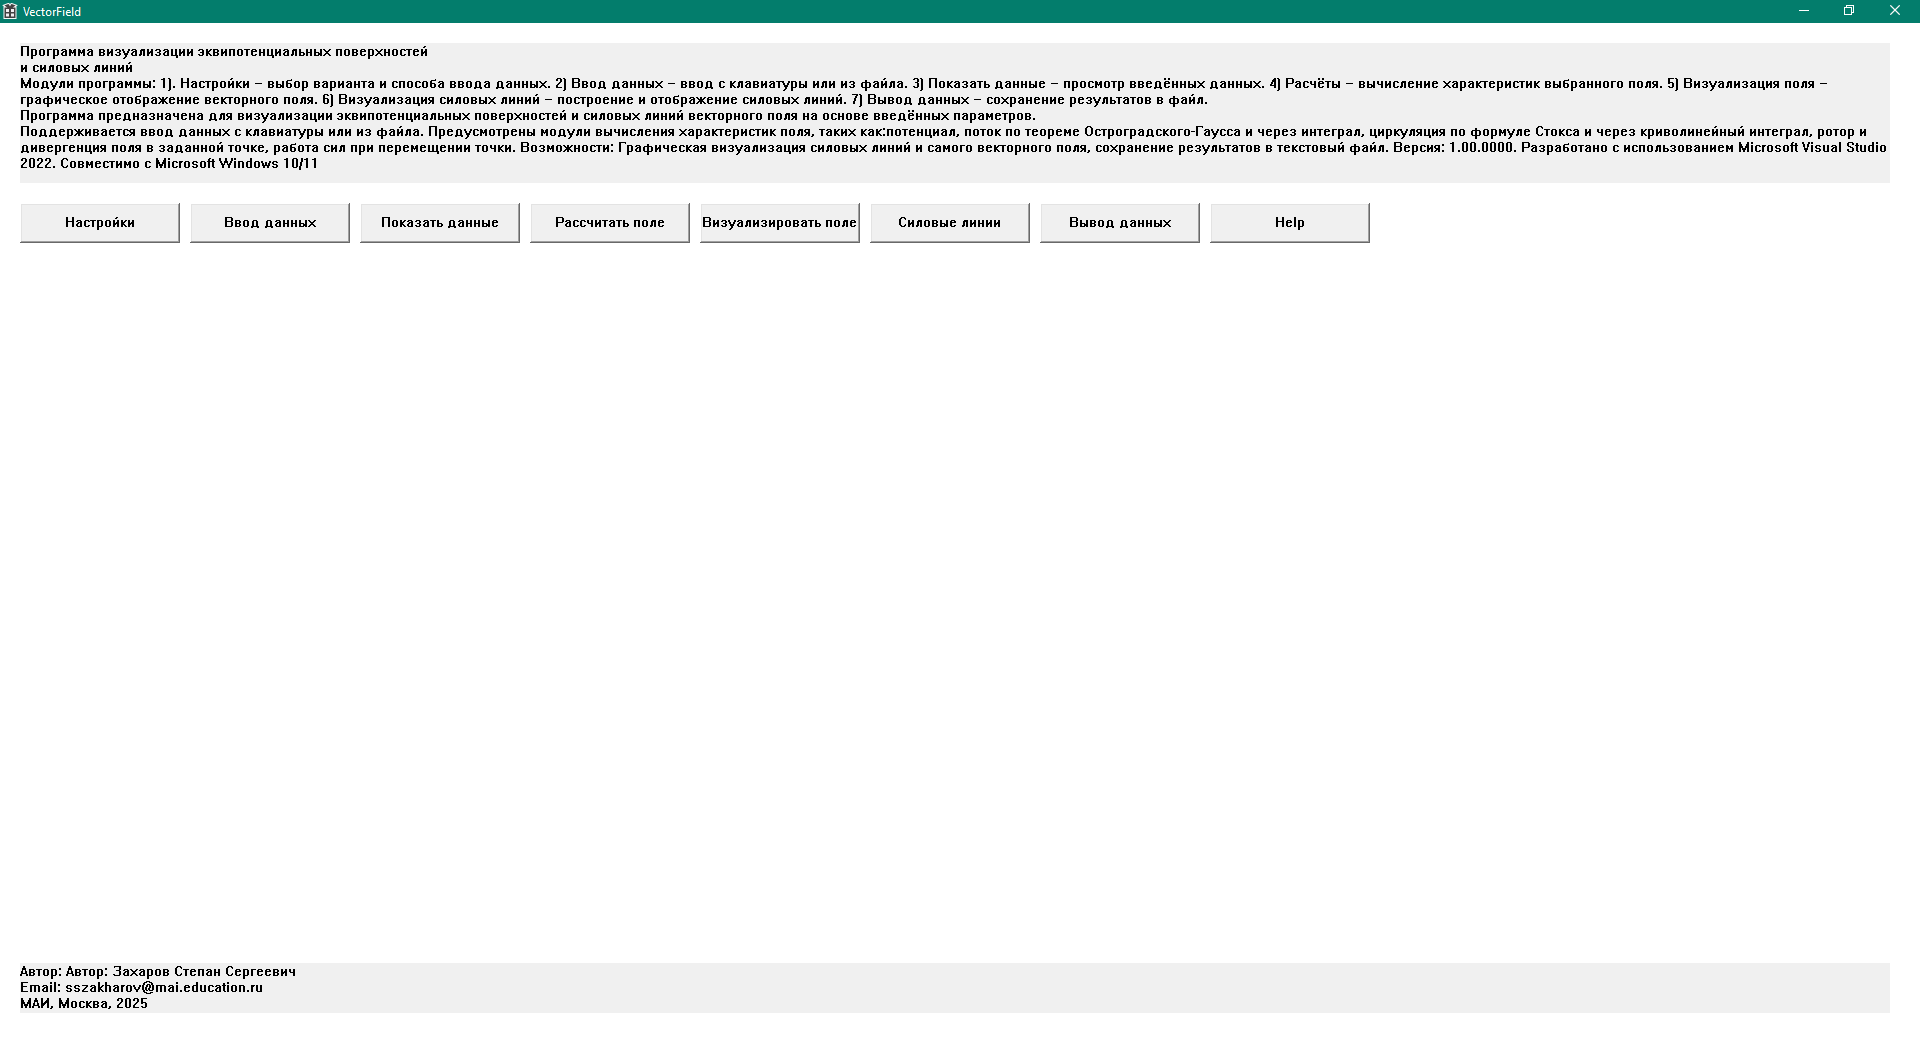
\includegraphics[width=0.95\linewidth]{pics/Главная кнопочная форма.png}
	\label{fig:1}
	\caption{Главная кнопочная форма}
\end{figure} 

В таблице 3.1 предоставлено описание идентификаторов главной кнопочной формы.

\begin{table}[H]
	\singlespacing
	\caption{Описание идентификаторов главной кнопочной формы}
	\label{table:1}
	\begin{tblr}{|[\rs]X[.1,c,m]|[\rs]X[1,c,m]|[\rs]X[1,c,m]|[\rs]X[1,c,m]|[\rs]}\hline[\rs]
		\textbf{№} & \textbf{Имя идентификатора} & \textbf{Описание идентификатора} & \textbf{Тип данных} \\\hline[\rs]
		1 & \texttt{Setting}      & Настройки программы & button \\\hline
		2 & \texttt{Input}      & Ввести данные & button \\\hline
		3 & \texttt{ShowInput}      & Показать введенные данные & button \\\hline
		4 & \texttt{Solve}    & Расчитать поле & button \\\hline
		5 & \texttt{VisualizeField} & Визуализировать поле& button \\\hline
		6 & \texttt{VisualizeLines} & Визуализировать силовые линии& button \\\hline
		7 & \texttt{Output} &Вывести данные& button \\\hline
		8 & \texttt{Exit}   & Выход из программы & button \\\hline
		9 & \texttt{Autor}   & Автор программы & char[256] \\\hline[\rs]
	\end{tblr}
\end{table}

После нажатия на кнопку \texttt{<Setting>} открывается окно с формой настроек, в которой пользователь может выбрать номер варианта и способ ввода данных. 

После нажатия на кнопку \texttt{<Input>} открывается окно для выбора файла с входными данными (в режиме ввода из файла) или окно для ввода данных с клавиатуры (в режиме ввода с клавиатуры).

После нажатия на кнопку \texttt{<ShowInput>} открывается окно с формой отображения выбранного сособа ввода и введенных данных.

После нажатия на кнопку \texttt{<Solve>} открывается окно с формой расчета поля, в котором отображаются результаты расчетов параметров поля. 

После нажатия на кнопку \texttt{<VisualizeField>} открывается окно с формой визуализации поля, в котором отображается (если возможно) результат визуализации эквипотенциальной поверхности,  в ином случае пользователю отображается сообщение о невозможности построения эквипотенциальной поверхности для выбранного поля.

После нажатия на кнопку \texttt{<VisualizeLines>} открывается окно с формой визуализации поля, в котором отображается (если возможно) результат визуализации силовых линий,  в ином случае пользователю отображается сообщение о невозможности построения силовых линий для выбранного поля.

После нажатия на кнопку \texttt{<Exit>} происходит выход из программы, сопровождающийся закрытием окна программы.

\subsubsection{Форма расчета поля}

Для вывода результатов расчета поля в форме отображены идентификаторы \texttt{<Comp1>}, \texttt{<Comp2>}, \texttt{<Comp3>}, \texttt{<PotVal>}, \texttt{<SphereRad>}, \texttt{<ClassOfField>}, \texttt{<FlowOG>}, \texttt{<FlowPI>}, \texttt{<CirculationStokes>}, \texttt{<CirculationKI>}, \texttt{<Rotor>}, \texttt{<WorkOfForces>}, \texttt{<BackToMenu>}. На рисунке 3.2 представлен вид формы расчета поля.

\begin{figure}[H]
	\centering
	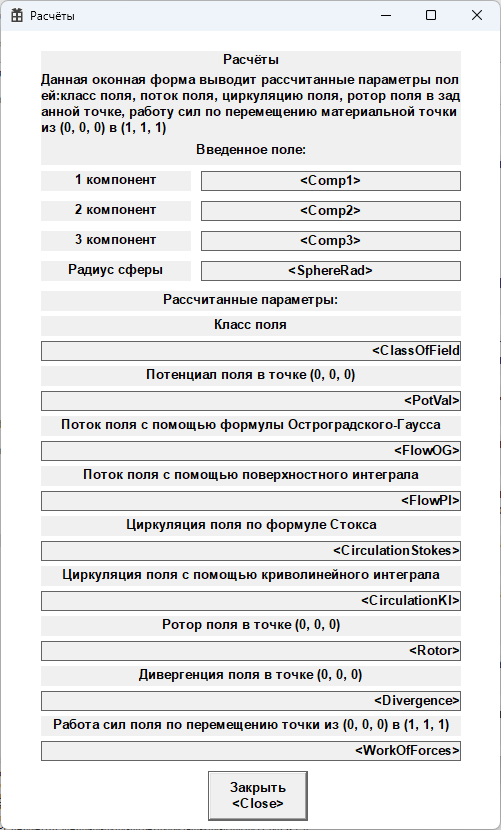
\includegraphics[width=0.7\linewidth]{pics/Форма расчета поля.png}
	\label{fig:3}
	\caption{Форма расчета поля}
\end{figure} 

В таблице 3.2 предоставлено описание идентификаторов формы расчета поля.

\begin{table}[H]
	\singlespacing
	\caption{Описание идентификаторов формы расчета поля}
	\label{table:2}
	\begin{tblr}{|[\rs]X[.1,c,m]|[\rs]X[1,c,m]|[\rs]X[1,c,m]|[\rs]X[1,c,m]|[\rs]}\hline[\rs]
		\textbf{№} & \textbf{Имя идентификатора} & \textbf{Описание идентификатора} & \textbf{Тип данных} \\\hline[\rs]
		1 & \texttt{Comp1} & Первый компонент поля & char[256] \\\hline
		2 & \texttt{Comp2}   & Второй компонент поля & char[256] \\\hline
		3 & \texttt{Comp3}   & Третий компонент поля & char[256] \\\hline
		4 & \texttt{PotVal}   & Значение потенциала эквипотенциальной поверхности & double \\\hline
		5 & \texttt{SphereRad}   & Радиус сферы & double \\\hline
		6 & \texttt{ClassOfField}   & Класс поля & char[256] \\\hline
		7 & \texttt{FlowOG}   & Поток поля по формуле Остроградского-Гаусса & double \\\hline
		8 & \texttt{FlowPI}   & Поток поля через поверхностный интеграл & double \\\hline
		9 & \texttt{CirculationStokes}   & Циркуляция поля по формуле Стокса & double \\\hline
		10 & \texttt{CirculationKI}   & Циркуляция поля через криволинейный интеграл & double \\\hline
		11 & \texttt{Rotor}   & Уравнение ротора выбранного поля & char[256] \\\hline
		12 & \texttt{RotorA}   & Ротор поля \( \vec a \) & double \\\hline
		13 & \texttt{RotorB}   & Ротор поля \( \vec b \) & double \\\hline
		14 & \texttt{WorkOfForces}   & Работа сил поля & double \\\hline
		15 & \texttt{BackToMenu}   & Возврат в главное меню & button \\\hline
		16 & \texttt{CompA\_X}   & Составляющая поля \( \vec a_x \) & double \\\hline
		17 & \texttt{CompA\_Y}   & Составляющая поля \( \vec a_y \) & double \\\hline
[\rs]
	\end{tblr}
\end{table}

\begin{table}[H]
	\singlespacing
	%\caption{Описание идентификаторов формы расчета поля}
	%\label{table:2}
	\begin{tblr}{|[\rs]X[.1,c,m]|[\rs]X[1,c,m]|[\rs]X[1,c,m]|[\rs]X[1,c,m]|[\rs]}\hline[\rs]
		%\textbf{№} & \textbf{Имя идентификатора} & \textbf{Описание идентификатора} & \textbf{Тип данных} \\\hline[\rs]

		18 & \texttt{CompA\_Z}   & Составляющая поля \( \vec a_z \) & double \\\hline
		19 & \texttt{DivergenceA}   &Дивергенция поля поля \( \vec a \) & double \\\hline
		20 & \texttt{ValueX}   & Переменная \( x \) & double \\\hline
		21 & \texttt{ValueY}   & Переменная \( y \) & double \\\hline
		22 & \texttt{ValueZ}   & Переменная \( z \) & double \\\hline
		23& \texttt{LoopABCD}   & Замкнутый контур \( ABCD \) & void \\\hline
		24& \texttt{SurfaceS}   & Поверхность \( S \) & void \\\hline
		25& \texttt{SurfaceS\_XY}   & Поверхность \( S_{xy} \) & void \\\hline
		26& \texttt{SurfaceS\_XY}   & Поверхность \( S_{xy} \) & void \\\hline
		27& \texttt{SurfaceS\_YZ}   & Поверхность \( S_{yz} \) & void \\\hline
		28& \texttt{SurfaceS\_XZ}   & Поверхность \( S_{xz} \) & void \\\hline
		29 & \texttt{XoY} & Координатная плоскость \( xOy \) & void \\\hline
		30 & \texttt{YoZ}   &Координатная плоскость \( yOz \)& void \\\hline
		31 & \texttt{XoZ}   & Координатная плоскость \( xOz \) & void \\\hline
		32 & \texttt{A\_PartDerivativeX}   & Частная производная  \( \frac{\partial a_x}{\partial x} \) & double \\\hline
		33 & \texttt{A\_PartDerivativeY}   & Частная производная  \( \frac{\partial a_y}{\partial y} \) & double \\\hline
		34 & \texttt{A\_PartDerivativeZ}   & Частная производная  \( \frac{\partial a_z}{\partial z} \) & double \\\hline
		35 & \texttt{A\_PartDerivativeZ\_Y}   & Частная производная  \( \frac{\partial a_z}{\partial y} \) & double \\\hline
		36 & \texttt{A\_PartDerivativeY\_Z}   & Частная производная  \( \frac{\partial a_y}{\partial z} \) & double \\\hline
		37 & \texttt{A\_PartDerivativeX\_Z}   & Частная производная  \( \frac{\partial a_x}{\partial z} \) & double \\\hline
		38 & \texttt{A\_PartDerivativeZ\_X}   & Частная производная  \( \frac{\partial a_z}{\partial x} \) & double \\\hline
[\rs]
	\end{tblr}
\end{table}

\begin{table}[H]
	\singlespacing
	%\caption{Описание идентификаторов формы расчета поля}
	%\label{table:2}
	\begin{tblr}{|[\rs]X[.1,c,m]|[\rs]X[1,c,m]|[\rs]X[1,c,m]|[\rs]X[1,c,m]|[\rs]}\hline[\rs]
		%\textbf{№} & \textbf{Имя идентификатора} & \textbf{Описание идентификатора} & \textbf{Тип данных} \\\hline[\rs]
		39 & \texttt{A\_PartDerivativeY\_X}   & Частная производная  \( \frac{\partial a_y}{\partial x} \) & double \\\hline
		40 & \texttt{A\_PartDerivativeX\_Y}   & Частная производная  \( \frac{\partial a_x}{\partial y} \) & double \\\hline
		41 & \texttt{B\_PartDerivativeX}   & Частная производная  \( \frac{\partial b_x}{\partial x} \) & double \\\hline
		42 & \texttt{B\_PartDerivativeY}   & Частная производная  \( \frac{\partial b_y}{\partial y} \) & double \\\hline
		43 & \texttt{B\_PartDerivativeZ}   & Частная производная  \( \frac{\partial b_z}{\partial z} \) & double \\\hline
		44 & \texttt{B\_PartDerivativeZ\_Y}   & Частная производная  \( \frac{\partial b_z}{\partial y} \) & double \\\hline
		45 & \texttt{B\_PartDerivativeY\_Z}   & Частная производная  \( \frac{\partial b_y}{\partial z} \) & double \\\hline
		46 & \texttt{B\_PartDerivativeX\_Z}   & Частная производная  \( \frac{\partial b_x}{\partial z} \) & double \\\hline
		47 & \texttt{B\_PartDerivativeZ\_X}   & Частная производная  \( \frac{\partial b_z}{\partial x} \) & double \\\hline
		48 & \texttt{B\_PartDerivativeY\_X}   & Частная производная  \( \frac{\partial b_y}{\partial x} \) & double \\\hline
		49 & \texttt{B\_PartDerivativeX\_Y}   & Частная производная  \( \frac{\partial b_x}{\partial y} \) & double \\\hline

		50 & \texttt{VectorI}   & Вектор \( \vec i \) & double \\\hline
		51 & \texttt{VectorJ}   & Вектор \( \vec j \) & double \\\hline
		52 & \texttt{VectorK}   & Вектор \( \vec k \) & double \\\hline

		53 & \texttt{FieldA}   & Вектор поля \( \vec a \) & double \\\hline
		54 & \texttt{FieldB}   & Вектор поля \( \vec a \) & double \\\hline

		55 & \texttt{DiffX}   & Дифференциал \( dx \) & double \\\hline
		56 & \texttt{DiffY}   & Дифференциал \( dy \) & double \\\hline
		57 & \texttt{DiffZ}   & Дифференциал \( dz \) & double \\\hline

		58 & \texttt{DiffS}   & Дифференциал \( dS \) & double \\\hline
		59 & \texttt{DiffV}   & Дифференциал \( dv \) & double \\\hline

		60 & \texttt{Rotor\_N}   & Ротор \( rot_n \) & double \\\hline
[\rs]
	\end{tblr}
\end{table}

\begin{table}[H]
	\singlespacing
	%\caption{Описание идентификаторов формы расчета поля}
	%\label{table:2}
	\begin{tblr}{|[\rs]X[.1,c,m]|[\rs]X[1,c,m]|[\rs]X[1,c,m]|[\rs]X[1,c,m]|[\rs]}\hline[\rs]
		%\textbf{№} & \textbf{Имя идентификатора} & \textbf{Описание идентификатора} & \textbf{Тип данных} \\\hline[\rs]

		61 & \texttt{CompB\_X}   & Составляющая поля \( \vec b \) по \( x \) & double \\\hline
		62 & \texttt{CompB\_Y}   & Составляющая поля \( \vec b \) по \( y \) & double \\\hline
		63 & \texttt{CompB\_Z}   & Составляющая поля \( \vec b \) по \( z \) & double \\\hline

		64 & \texttt{IIIntT}   & Тройной интеграл \( \iiint\limits_T \) & double \\\hline

		65 & \texttt{IIIntT}   & Тройной интеграл \( \iiint\limits_T \) & double \\\hline
		66 & \texttt{Int0-X}   & Интеграл \( \int_0^x \) & double \\\hline
		67 & \texttt{Int0-Y}   & Интеграл \( \int_0^y \) & double \\\hline
		68 & \texttt{Int0-Z}   & Интеграл \( \int_0^z \) & double \\\hline
		69 & \texttt{IIntS}   & Тройной интеграл \( \iint\limits_S \) & double \\\hline
		70 & \texttt{OIntABCD+}   & Контурный интеграл \( \oint\limits_{ABCD_+} \) & double \\\hline

		71 & \texttt{OIntABCD+}   & Контурный интеграл \( \oint\limits_{ABCD_+} \) & double \\\hline

		72 & \texttt{PartDerivPot\_X}   & Частная производная \( \varphi'_x \) & double \\\hline
		73 & \texttt{PartDerivPot\_Y}   & Частная производная \( \varphi'_y \) & double \\\hline
		74 & \texttt{PartDerivPot\_Z}   & Частная производная \( \varphi'_z\) & double \\\hline

		75 & \texttt{PotVal(0,0,0)}   & Потенциал поля \( \varphi(0, 0, 0) \) & double \\\hline
		76 & \texttt{PotVal(1,1,1)}   & Потенциал поля \( \varphi(1, 1, 1) \) & double \\\hline
[\rs]
	\end{tblr}
\end{table}

Алгоритм расчета:
\begin{enumerate}[label=\arabic*.,ref=\arabic*]
	\item определить класс поля \texttt{<ClassOfFieldA>}:
	\begin{enumerate}[label=\arabic*),ref=\arabic*]
		\item вычислить дивергенцию поля \texttt{<DivergenceA>}: \texttt{<Divergence>} =  \texttt{<A\_PartDerivativeX>} +  \texttt{<A\_PartDerivativeY>} +  		\texttt{<A\_PartDerivativeZ>};
		\item вычислить ротор: \texttt{<RotorA>}:  \texttt{<RotorA>} = (\texttt{<A\_PartDerivativeZ\_Y>} --- \texttt{<A\_PartDerivativeY\_Z>})\texttt{<VectorI>} + 
(\texttt{<A\_PartDerivativeX\_Z>} --- \texttt{<A\_PartDerivativeZ\_X>})\texttt{<VectorJ>} + (\texttt{<A\_PartDerivativeY\_X>} ---  \texttt{<A\_PartDerivativeX\_Y>})\texttt{<VectorK>};
	\end{enumerate}

	\item Определить поток поля \texttt{<FlowOG>} и \texttt{<FlowPI>}:
	\begin{enumerate}[label=\arabic*),ref=\arabic*]
		\item \texttt{<FlowOG>} =  (\texttt{<A\_PartDerivativeX>} +  \texttt{<A\_PartDerivativeY>} +  \texttt{<A\_PartDerivativeZ>})\texttt{<DiffV>};

		\item \texttt{<FlowPI>} = \texttt{<IIIntT>}( \texttt{<ValueX>}\texttt{<ValueZ>}\texttt{<DiffY>}\texttt{<DiffZ>}\\ + 
\texttt{<ValueX>}\texttt{<ValueY>}\texttt{<DiffZ>}\texttt{<DiffX>} +
\texttt{<ValueY>}\texttt{<ValueZ>}\texttt{<DiffX>}\texttt{<DiffY>}); 
	\end{enumerate}


	\item Вычислить циркуляцию по контуру \texttt{<LoopABCD>}: 
	\begin{enumerate}[label=\arabic*),ref=\arabic*]
		\item \texttt{<CirculationStokes>} = \texttt{<IIntS>} (\texttt{<RotorN>}\texttt{<FieldA>} \texttt{<DiffS>});

		\item \texttt{<CirculationKI>} =  \texttt{<OIntABCD+>}  (\texttt{<CompA\_X>}\texttt{<DiffX>}  + \texttt{<CompA\_Y>}\texttt{<DiffY>} + \texttt{<CompA\_Z>}\texttt{<DiffZ>} );
	\end{enumerate}

	\item Изучить поле \texttt{FieldB}:
	\begin{enumerate}[label=\arabic*),ref=\arabic*]
		\item Вычислить \texttt{<RotorB>}: \texttt{<RotorB>} = \texttt{<RotorA>} = (\texttt{<B\_PartDerivativeZ\_Y>} --- \texttt{<B\_PartDerivativeY\_Z>})\texttt{<VectorI>} + 
(\texttt{<B\_PartDerivativeX\_Z>} --- \texttt{<B\_PartDerivativeZ\_X>})\texttt{<VectorJ>} + (\texttt{<B\_PartDerivativeY\_X>} ---  \texttt{<B\_PartDerivativeX\_Y>})\texttt{<VectorK>};

		\item Вычислить \texttt{<PotVal>}: \texttt{<PotVal>} = \texttt{<Int0-X>}(\texttt{<CompB\_X>}\texttt{<DiffX>}) + 
\texttt{<Int0-Y>}(\texttt{<CompB\_Y>}\texttt{<DiffY>}) + 
\texttt{<Int0-Z>}(\texttt{<CompB\_Z>}\texttt{<DiffZ>});

		\item Выполнить сравнение: \texttt{<PartDerivPot\_X>} == \texttt{<CompB\_X>}, \texttt{<PartDerivPot\_Y>} == \texttt{<CompB\_Y>}, \texttt{<PartDerivPot\_Z} == \texttt{<CompB\_Z>};
	\end{enumerate}

		\item Вычислить работу поля \texttt{<WorkOfForces>}: \texttt{<WorkOfForces>} = \texttt{<PotVal(1,1,1)>} --- \texttt{<PotVal(0,0,0)>};
	\end{enumerate}
%\end{enumerate}

По нажатию на кнопку \texttt{<BackToMenu>} происхоодит закрытие оконной формы и возврат в главную оконную форму с главным меню.

\vspace{0.8cm}
\subsubsection{Форма с визуализацией эквипотенциальных поверхностей}

В форме с визуализацией отображается эквипотенциальная поверхность и силовые линии поля в обалсти \texttt{<Vizualization>}. На рисунке 3.3 представлен вид формы с визуализацией.

\begin{figure}[H]	
	\centering
	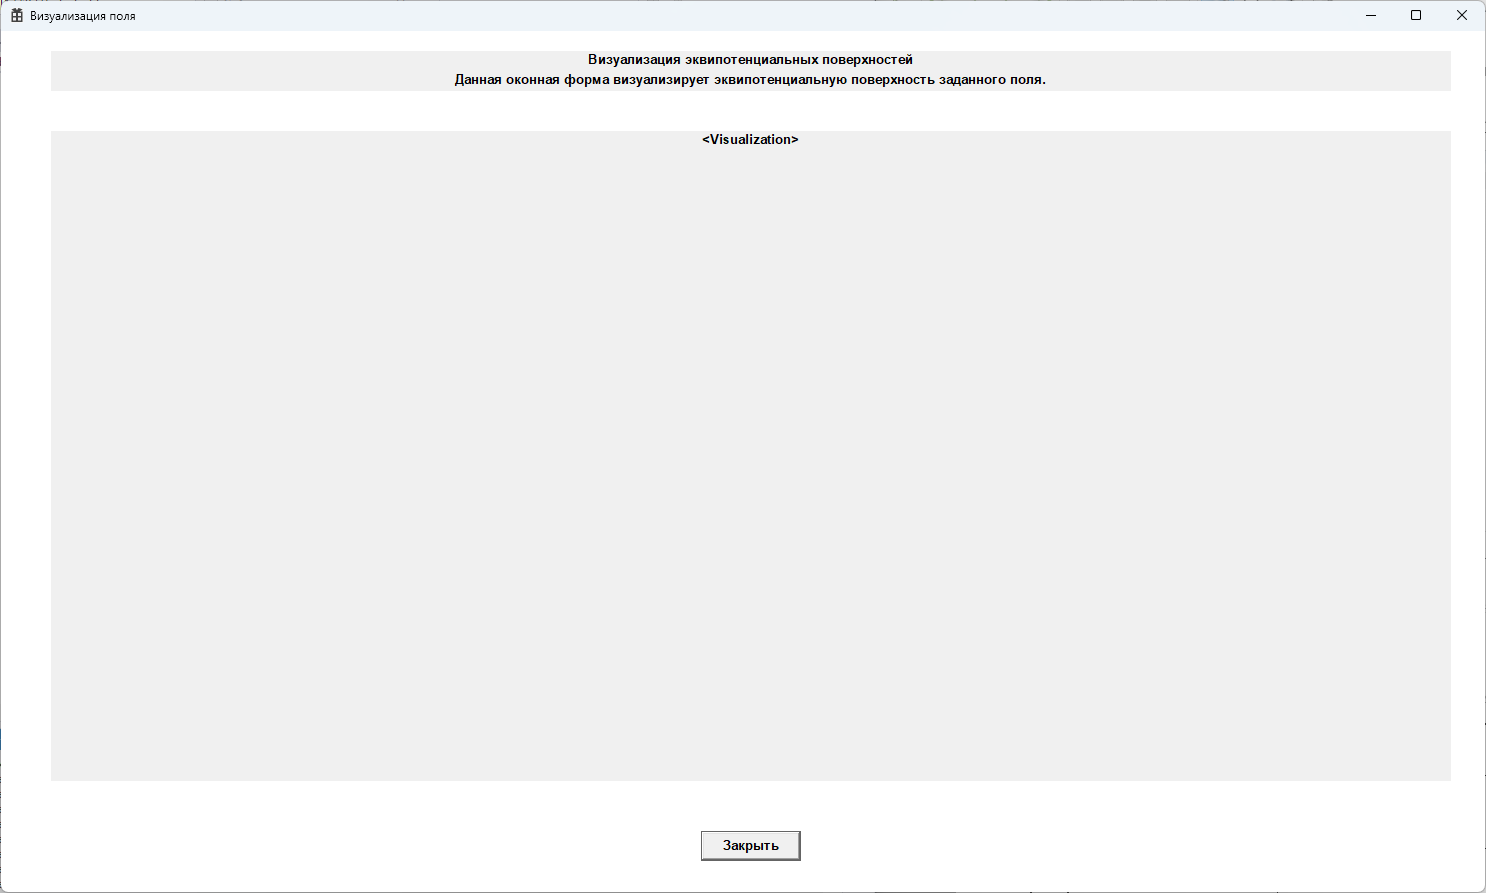
\includegraphics[width=0.95\linewidth]{pics/Визуализация поля.png}
	\label{fig:2}
	\caption{Форма с визуализацией эквипотенциальной поверности поля}
\end{figure} 

В таблице 1.3 предоставлено описание идентификаторов формы с визуализацией эквипотенциальной поверхости поля.

\begin{table}[H]
	\singlespacing
	\caption{Описание идентификаторов формы с визуализацией эквипотенциальной поверхности}
	\label{table:3}
	\begin{tblr}{|[\rs]X[.1,c,m]|[\rs]X[1,c,m]|[\rs]X[1,c,m]|[\rs]X[1,c,m]|[\rs]}\hline[\rs]
		\textbf{№} & \textbf{Имя идентификатора} & \textbf{Описание идентификатора} & \textbf{Тип данных} \\\hline[\rs]
		1 & \texttt{Vizualization}      & Визуализация эквипотенциальной поверхности & image \\\hline
		2 & \texttt{BackToMenu}      & Возврат в главное меню & button \\\hline[\rs]
	\end{tblr}
\end{table}

После открытия окна в форме визуализации \texttt{<Visualization>} визуализируется эквипотенциальная поверхность поля.

По нажатию на кнопку \texttt{<BackToMenu>} происходит  закрытие оконной формы и возврат в главную оконную форму с главным меню.

\vspace{0.8cm}
\subsubsection{Форма с визуализацией силовых линий}

В форме с визуализацией отображаются силовые линии поля в области \texttt{<Vizualization>}. На рисунке 3.3 представлен вид формы с визуализацией.

\begin{figure}[H]	
	\centering
	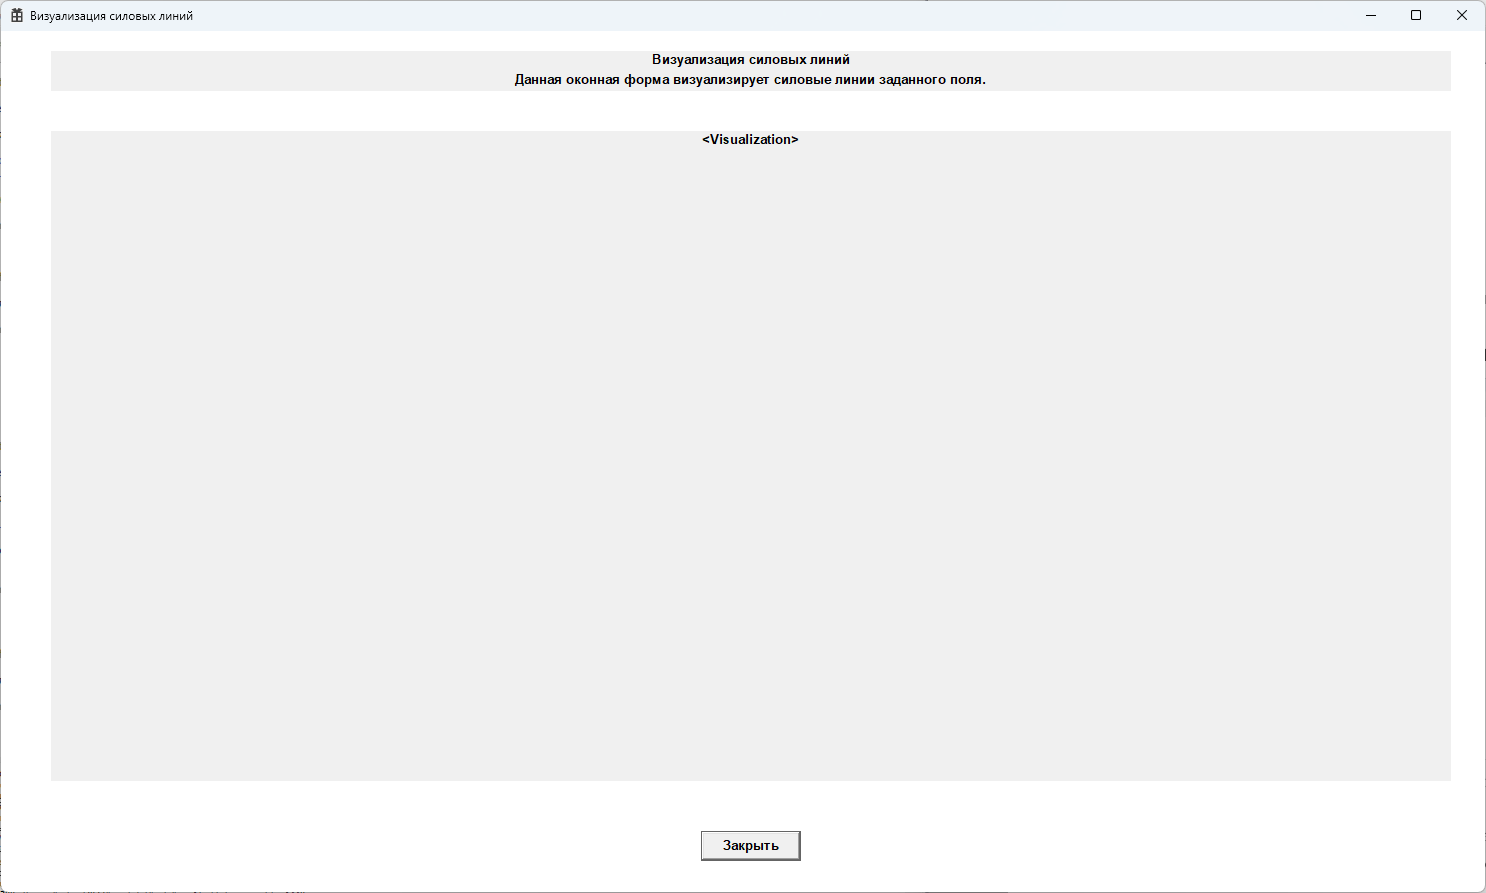
\includegraphics[width=0.95\linewidth]{pics/Визуализация силовых линий.png}
	\label{fig:2}
	\caption{Форма с визуализацией силовых линий}
\end{figure} 

В таблице 3.4  предоставлено описание идентификаторов формы с визуализацией силовых линий.

\begin{table}[H]
	\singlespacing
	\caption{Описание идентификаторов формы с визуализацией силовых линий}
	\label{table:3}
	\begin{tblr}{|[\rs]X[.1,c,m]|[\rs]X[1,c,m]|[\rs]X[1,c,m]|[\rs]X[1,c,m]|[\rs]}\hline[\rs]
		\textbf{№} & \textbf{Имя идентификатора} & \textbf{Описание идентификатора} & \textbf{Тип данных} \\\hline[\rs]
		1 & \texttt{Vizualization}      & Визуализация силовых линий поля & image \\\hline
		2 & \texttt{BackToMenu}      & Возврат в главное меню & button \\\hline[\rs]
	\end{tblr}
\end{table}

После открытия окна в форме визуализации \texttt{<Visualization>} визуализируются силовые линии поля.

По нажатию на кнопку \texttt{<BackToMenu>} происходит  закрытие оконной формы и возврат в главную оконную форму с главным меню.

\subsubsection{Форма с настройками}

На форме с настройками отображена настройка метода инициализации векторных полей и выбор номера варианта. На рисунке 3.5 представлен вид формы с настройками.


\begin{figure}[H]	
	\centering
	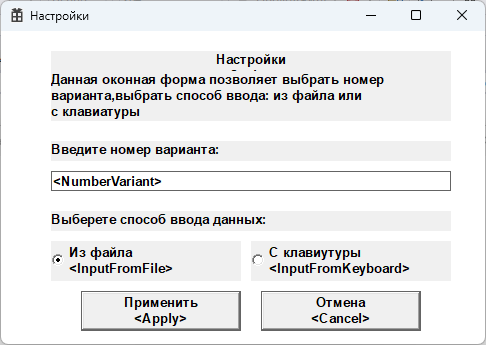
\includegraphics[width=0.8\linewidth]{pics/Настройки.png}
	\label{fig:2}
	\caption{Форма с настройками}
\end{figure} 

В таблице 3.4 предоставлено описание идентификаторов формы с настройками.

\begin{table}[H]
	\singlespacing
	\caption{Описание идентификаторов формы с настройками}
	\label{table:3}
	\begin{tblr}{|[\rs]X[.1,c,m]|[\rs]X[1,c,m]|[\rs]X[1,c,m]|[\rs]X[1,c,m]|[\rs]}\hline[\rs]
		\textbf{№} & \textbf{Имя идентификатора} & \textbf{Описание идентификатора} & \textbf{Тип данных} \\\hline[\rs]
		1 & \texttt{NumberVarian}      & Номер варианта & char[256] \\\hline
		2 & \texttt{InputFromFile}      & Флаг считывания из файла & bool \\\hline
		3 & \texttt{InputFromKeyboard} & Флаг считывания из с клавиатуры & bool \\\hline
		4 & \texttt{Apply}      & Применить изменения & button \\\hline
		5 & \texttt{Cancel}      & Отменить изменения & button \\\hline[\rs]
	\end{tblr}
\end{table}

В текстовом поле \texttt{<NumberVariant>} необходимо вписать номер варианта.

Необходимо выбрать один из двух флагов \texttt{<InputFromFile>} или \texttt{<InputFromKeyboard>} для выбора способа ввода.

При нажатии на кнопку \texttt{<Apply>} применяются текущие выбранные настройки. 

При нажатии на кнопку \texttt{<Cancel>} увнесенные изменения удаляются, восстанавливается предыдущая врсия настроек.

\section{Описание алгоритма и функционирования программы}

\subsection{Функция основной программы}

\begin{figure}[H]	
	
\includegraphics[width=0.95\linewidth]{pics/4.png}
	\label{fig:2}
	\caption{Форма с информацией о программе}
\end{figure} 

\pagebreak

\subsection{Список символов главной функции}

\texttt{1A1} -- Терминатор начала главной функции программы.
 
\texttt{1B1} -- Программа инициализирует модули: главное окно программы, внутренние поля, интерфейс программы.

\texttt{1C1} -- Начало основного цикла программы.

\texttt{1D1} -- Проверка условия: отправлено ли сообщение о выходе из программы. Если <<да>>, то основной цикл программы заканчивается, переход к \texttt{1E3}. Если <<нет>>, то главный поток продолжает выполнение главного цикла.

\texttt{1E1} -- Проверка условия: нажата ли кнопка. Если <<нет>>, то главный поток идет в конец цикла, переход к \texttt{1D3}. Если <<да>>, то главный поток продолжает выполнение главного цикла.

\texttt{1F1} -- Определение класса поля A.

\texttt{1A2} -- Нахождение потока поля A с помощью формулы Остроградского-Гаусса.

\texttt{1B2} -- Нахождение потока поля A с помощью поверхностного интеграла.

\texttt{1C2} -- Нахождение циркуляции поля A по формуле стокса.

\texttt{1D2} -- Нахождение циркуляции поля A через криволинейный интеграл.

\texttt{1E2} -- Нахождение ротора поля B.

\texttt{1F2} -- Вычисление работы сил поля B по перемещению материальной точки из точки (0, 0, 0) в точку (1, 1, 1).

\texttt{1A3} -- Вывод полученных результатов расчета на экран.

\texttt{1B3} -- Визуализация рассчитанных эквипотенциальных поверхностей на экране.

\texttt{1C3} -- Визуализация рассчитанных силовых линий на экране.

\texttt{1D3} -- Конец основного цикла программы.

\texttt{1E3} -- Терминатор конца главной функции программы.

\pagebreak

\subsection{Функция расчетов параметров поля}

\begin{figure}[H]	
	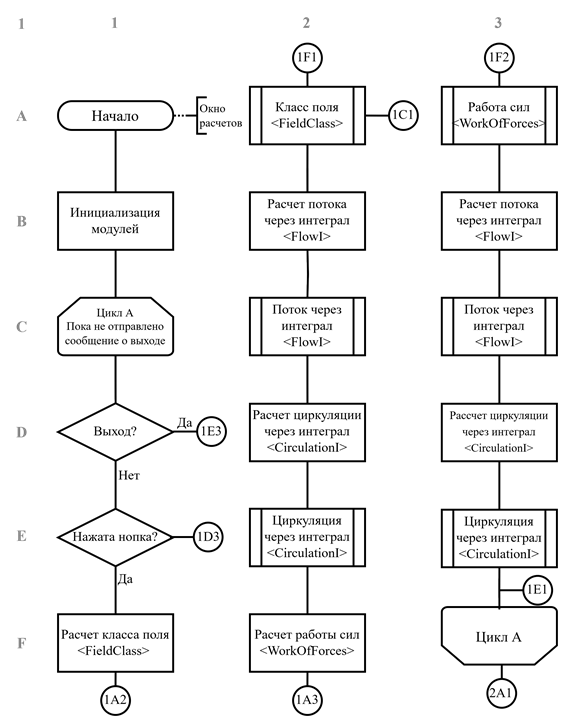
\includegraphics[width=0.95\linewidth]{pics/5.png}
	\label{fig:2}
	\caption{Форма с информацией о программе}
\end{figure} 


\begin{figure}[H]	
	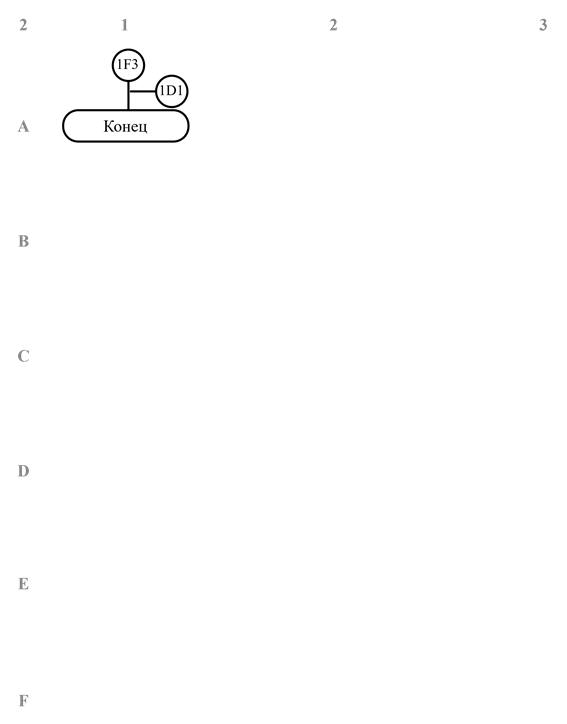
\includegraphics[width=0.95\linewidth]{pics/6.png}
	\label{fig:2}
	\caption{Форма с информацией о программе}
\end{figure} 

\pagebreak

\subsection{Список символов функции расчетов параметров поля}

\texttt{1A1} -- Терминатор начала главной функции программы.
 
\texttt{1B1} -- Функция инициализирует модули: окно расчетов, переменные для расчетов.

\texttt{1C1} -- Начало основного цикла функции.

\texttt{1D1} -- Проверка условия: отправлено ли сообщение о выходе из функции. Если <<да>>, то основной цикл программы заканчивается, переход к \texttt{1E3}. Если <<нет>>, то главный поток продолжает выполнение главного цикла.

\texttt{1E1} -- Проверка условия: нажата ли кнопка. Если <<нет>>, то главный поток идет в конец цикла, переход к \texttt{1D3}. Если <<да>>, то главный поток продолжает выполнение главного цикла.

\texttt{1F1} -- Расчет класса поля A.

\texttt{1А2} -- Вывод класса поля A на экран.

\texttt{1B2} --  Расчет потока поля A с помощью формулы Остроградского-Гаусса.

\texttt{1C2} -- Вывод потока поля A с помощью формулы Остроградского-Гаусса на экран.

\texttt{1D2} --  Расчет потока поля A с помощью поверхностного интеграла.

\texttt{1E2} -- Вывод потока поля A с помощью поверхностного интеграла на экран.

\texttt{1F2} --  Расчет циркуляции поля A по формуле Стокса.

\texttt{1A3} -- Вывод циркуляции поля A по формуле Стокса на экран.

\texttt{1B3} --  Расчет циркуляции поля A через криволинейный интеграл.

\texttt{1C3} -- Вывод циркуляции поля A через криволинейный интеграл на экран.

\texttt{1D3} --  Расчет ротора поля B.

\texttt{1E3} -- Вывод ротора поля B на экран.

\texttt{1F3} --  Расчет работы сил поля B по перемещению материальной точки из точки (0, 0, 0) в точку (1, 1, 1).

\texttt{1F2} -- Вывод работы сил поля B по перемещению материальной точки из точки (0, 0, 0) в точку (1, 1, 1) на экран.

\texttt{1D3} -- Конец основного цикла программы.

\texttt{1E3} -- Терминатор конца главной функции программы.

\pagebreak

\subsection{Возможные взаимодействия программы с другими программами}

В ходе работы программа взаимодействует со следующими внешними библиотеками:
\begin{enumerate}[itemindent=\parindent]
\item <windows.h> -- основная библиотека, в которой объявляются функции, предоставляющие интерфейс доступа к Windows API;
	\item <string> -- определяет шаблон basic\_string класса контейнера и различные вспомогательные шаблоны;
	\item <iostream> -- объявляет объекты, управляющие чтением из стандартных потоков и записью в них;
	\item <cmath> -- включает заголовок <math.h> стандартной библиотеки C и добавляет связанные имена в std пространство имен;
	\item <functional> -- определяет функции стандартной библиотеки C++, которые помогают создавать объекты функций;
\end{enumerate}

\section{Описание и обоснование выбора метода организации входных данных}

Описание входных данных программы приведены в разделе <<Входные данные>> программного документа <<Описание применения>>.

\section{Описание и обоснование выбора метода организации выходных данных}

Описание выходных данных программы приведены в разделе <<Выходные данные>> программного документа <<Описание применения>>.

\section{Постановка задачи на разработку программы тестирования}

\subsection{Идентификаторы экранных форм}

\subsubsection{Главная кнопочная форма}

На главной кнопочной форме отображена информация о программе тестирования и расположены кнопки главного меню. На рисунке 3.6 представлен вид главной кнопочной формы.

\begin{figure}[H]	
	\centering
	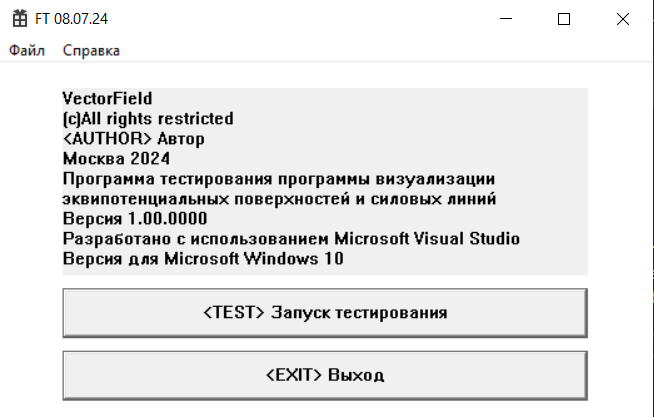
\includegraphics[width=0.8\linewidth]{pics/Главная кнопочная форма тестирования.png}
	\label{fig:1}
	\caption{Главная кнопочная форма}
\end{figure} 

В таблице 1.1 предоставлено описание идентификаторов главной кнопочной формы.

\begin{table}[H]
	\singlespacing
	\caption{Описание идентификаторов главной кнопочной формы}
	\label{table:1}
	\begin{tblr}{|[\rs]X[.1,c,m]|[\rs]X[1,c,m]|[\rs]X[1,c,m]|[\rs]X[1,c,m]|[\rs]}\hline[\rs]
		\textbf{№} & \textbf{Имя идентификатора} & \textbf{Описание идентификатора} & \textbf{Тип данных} \\\hline[\rs]
		1 & \texttt{TEST}   & Запуск тестирования & button \\\hline
		2 & \texttt{EXIT}   & Выход из программы & button \\\hline[\rs]
	\end{tblr}
\end{table}

После нажатия на оператор \texttt{<TEST>} происходит открытие окна с формой с отчетом тестирования, в которой отображается информация о проведенном тестировании данных из файла. 

При нажатии на оператор \texttt{<EXIT>} происходит выход из программы, сопровождающийся закрытием окна программы.

\subsubsection{Форма с отчетом тестирования}

Для вывода результатов тестирования в форме отображен идентификатор \texttt{<REPORT>}. На рисунке 3.7 представлен вид формы с отчетом тестирования.

\begin{figure}[H]	
	\centering
	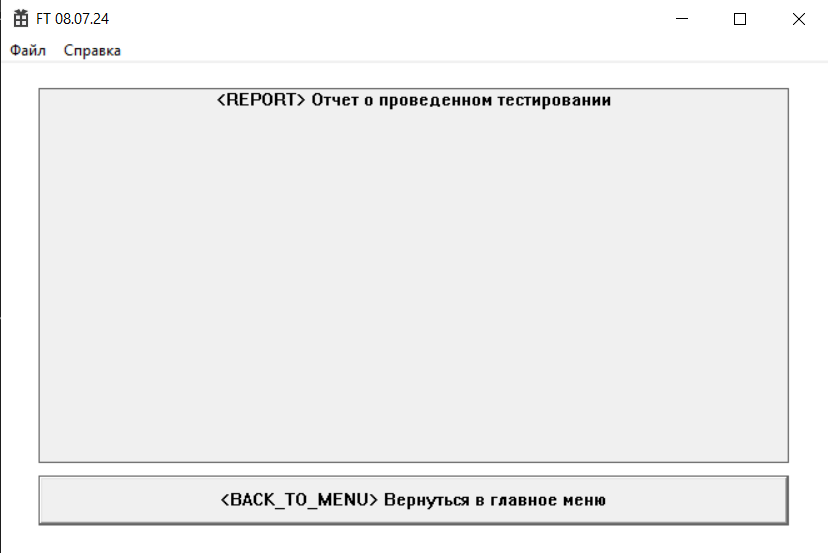
\includegraphics[width=0.95\linewidth]{pics/Форма с отчетом.png}
	\label{fig:3}
	\caption{Форма с отчетом тестирования}
\end{figure} 

В таблице 1.2 предоставлено описание идентификаторов формы с отчетом тестирования.

\begin{table}[H]
	\singlespacing
	\caption{Описание идентификаторов формы с отчетом тестирования}
	\label{table:2}
	\begin{tblr}{|[\rs]X[.1,c,m]|[\rs]X[1,c,m]|[\rs]X[1,c,m]|[\rs]X[1,c,m]|[\rs]}\hline[\rs]
		\textbf{№} & \textbf{Имя идентификатора} & \textbf{Описание идентификатора} & \textbf{Тип данных} \\\hline[\rs]
		1 & \texttt{REPORT} & Отчет о проведенном тестировании & char[256] \\\hline
		2 & \texttt{BACK\_TO\_MENU}   & Выход в главное меню & void \\\hline[\rs]
	\end{tblr}
\end{table}

\section{Описание и обоснование выбора состава технических средств}

В состав технических средств входит: \texttt{IBM}-совместимый персональный компьютер (ПЭВМ), включающий в себя:
\begin{enumerate}[label=\asbuk*),ref=\asbuk*]
	\item Процессор \texttt{Intel Core i5} 2-ого поколения; %000
	\item Оперативную память объемом, 256 Мб;
	\item Графический процессор \texttt{Intel HD Graphics 3000};
	\item Свободного места для хранения 64 Мб;
	\item Периферийные устройства такие как клавиатура, монитор с разрешением не менее 1280 точек в ширину и 720 точек в высоту.
\end{enumerate}

\section{Описание и обоснование выбора состава программных средств}

Для обеспечения функционирования программы на компьютере, на котором будет эксплуатироваться данный программный продукт, должно быть установлено следующее программное обеспечение:
\\
Наименование программы: C++.
\\
Обозначение программы: C++.
\\
Версия программного изделия: 15.0

\chapter{ОЖИДАЕМЫЕ ТЕХНИКО-ЭКОНОМИЧЕСКИЕ ПОКАЗАТЕЛИ}
Ожидаемые технико-экономические показатели не рассчитываются.

\pagebreak

\label{lastpage}

%\newcounter{totalpages}
%\setcounter{totalpages}{\pageref{lastpage}}
%\addtocounter{totalpages}{5}


\addcontentsline{toc}{chapter}{Лист регистрации изменений}
\renewcommand{\headrulewidth}{0pt}
\fontsize{3.5mm}{3mm}\selectfont
\noindent\begin{tblr}{colspec={|[\rs]p{8mm,c}|X[20,c]|X[20,c]|X[20,c]|X[20,c]|X[20,c]|X[25,c]|X[25,c]|X[15,c]|X[12,c]|[2pt]},
             rows   = {5mm},
             row{1} = {10mm,m},
             row{2} = {5mm,m},
             row{3} = {20mm,m},
             rowsep = 0pt,colsep = 0pt,
             vline{2-10} = {2-3}{\rs}
}\hline[\rs]
\SetCell[c=10]{c} {\fontsize{7mm}{0mm}\selectfont Лист регистрации изменений} &&&&&&&&&&& \\\hline[\rs]
\SetCell[c=5]{c} {\small Номера листов (страниц)} &&&&& \SetCell[r=2]{c} Всего листов (страниц) в документе & \SetCell[r=2]{c} № документа & \SetCell[r=2]{c} {Входящий № сопроводи-\\тельного  документа и дата} & \SetCell[r=2]{c} Подп. & \SetCell[r=2]{c} Дата \\\hline[\rs]
Изм & {Изменен-\\ных} & {Заменен-\\ных} & Новых & {Анулиро-\\ванных} &&&&& \\\hline[\rs]
&&&&&&&&&&& \\ \hline
&&&&&&&&&&& \\ \hline
&&&&&&&&&&& \\ \hline
&&&&&&&&&&& \\ \hline
&&&&&&&&&&& \\ \hline
&&&&&&&&&&& \\ \hline
&&&&&&&&&&& \\ \hline
&&&&&&&&&&& \\ \hline
&&&&&&&&&&& \\ \hline
&&&&&&&&&&& \\ \hline
&&&&&&&&&&& \\ \hline
&&&&&&&&&&& \\ \hline
&&&&&&&&&&& \\ \hline
&&&&&&&&&&& \\ \hline
&&&&&&&&&&& \\ \hline
&&&&&&&&&&& \\ \hline
&&&&&&&&&&& \\ \hline
&&&&&&&&&&& \\ \hline
&&&&&&&&&&& \\ \hline
&&&&&&&&&&& \\ \hline
&&&&&&&&&&& \\ \hline
&&&&&&&&&&& \\ \hline
&&&&&&&&&&& \\ \hline
&&&&&&&&&&& \\ \hline
&&&&&&&&&&& \\ \hline
&&&&&&&&&&& \\ \hline
&&&&&&&&&&& \\ \hline
&&&&&&&&&&& \\ \hline
&&&&&&&&&&& \\ \hline
&&&&&&&&&&& \\ \hline
&&&&&&&&&&& \\ \hline
&&&&&&&&&&& \\ \hline
&&&&&&&&&&& \\ \hline
&&&&&&&&&&& \\ \hline
&&&&&&&&&&& \\ \hline
&&&&&&&&&&& \\ \hline
&&&&&&&&&&& \\ \hline
&&&&&&&&&&& \\ \hline
&&&&&&&&&&& \\ \hline
&&&&&&&&&&& \\ \hline[\rs]
\end{tblr}

\end{document}